\documentclass[a4paper,12pt,oneside]{report}

\usepackage{report}

\begin{document}

\title{Interim Report:\\Ontology-based Data Integration}
\author{Jizhou Che}
\submitdate{December 2020}
\degree{BSc Computer Science with Artificial Intelligence}
\studentid{20032291}
\studentemail{scyjc1@nottingham.edu.cn}
\supervisor{Dr. Heshan Du}

\normallinespacing
\maketitle

% Delete the two declaration sentences in thesis.sty if not applicable. 

\preface

% \addcontentsline{toc}{chapter}{Abstract}

\begin{abstract}

Giving a short overview of the work in your project.

\end{abstract}


% \cleardoublepage

\addcontentsline{toc}{chapter}{Acknowledgements}

\begin{acknowledgements}

Acknowledgements here. \cite{Li2017}

\end{acknowledgements}


% There is a maximum limit of 15,000 words without exceeding 40 pages (A4 sides) for the main body of the dissertation that will be submitted in PDF. This limitation includes the bibliography and excludes cover/front pages (e.g., abstract, acknowledgement, table of contents) and excludes the appendices, listing of any codes or any other supporting documentation.
% Note: Your dissertation should not exceed the word and page limits. You do not have to use up your word limit to get a good grade; never `pad out' your dissertation, this will only annoy the markers.

\body

\chapter{Introduction}

Setting out the aims and objectives of your project, explaining the overall intention of the project and specific steps that will be taken to achieve that intention.

\section{Motivation}

Explaining the problem being solved.


\section{Aims and Objectives}

Aims and Objectives here.


\section{Description of the work}

Explaining what your project is meant to achieve, how it is meant to function, perhaps even a functional specification.


\chapter{Related Work}

This chapter outlines the major studies in ontology matching methodologies and specifically targets the field of instance matching, by providing a high-level classification with respect to their main characteristics. Based on these methods, the structures of the most recent and impactful matching systems are introduced along with their latest evaluation results.


\section{Classification of Techniques}

Many approaches have been proposed for the classification of ontology matching techniques. For example, one way is to look at the input, process and output dimensions of the algorithms \cite{euzenat2013d}. Characteristics such as the representation models accepted as input, the type of context used, and the cardinality of output alignments are taken into account. Another way is to distinguish between local methods that directly target the properties of the entities, such as string comparison, and globals methods that investigate into the structures that hold the entities together, such as graph segments. The most accepted classification method was proposed by Jérôme Euzenat and Pavel Shvaiko, which considers the different sources and interpretations of the input information, and further classify them with respect to how they are being processed \cite{euzenat2013d}. Other classification methods from different inspirations exist \cite{DBLP:conf/swb/Ehrig2007,DBLP:conf/icde/MadhavanBDH05}, but the ideas are generally similar.
\\\\
Based on the fundamental differences identified in the above mentioned approaches, this section describes a classification method focusing on the algorithmic characteristics of the local methodologies used for instance matching. The proposed classification is shown in Figure \ref{fig:techniques}.

\begin{figure}[ht]
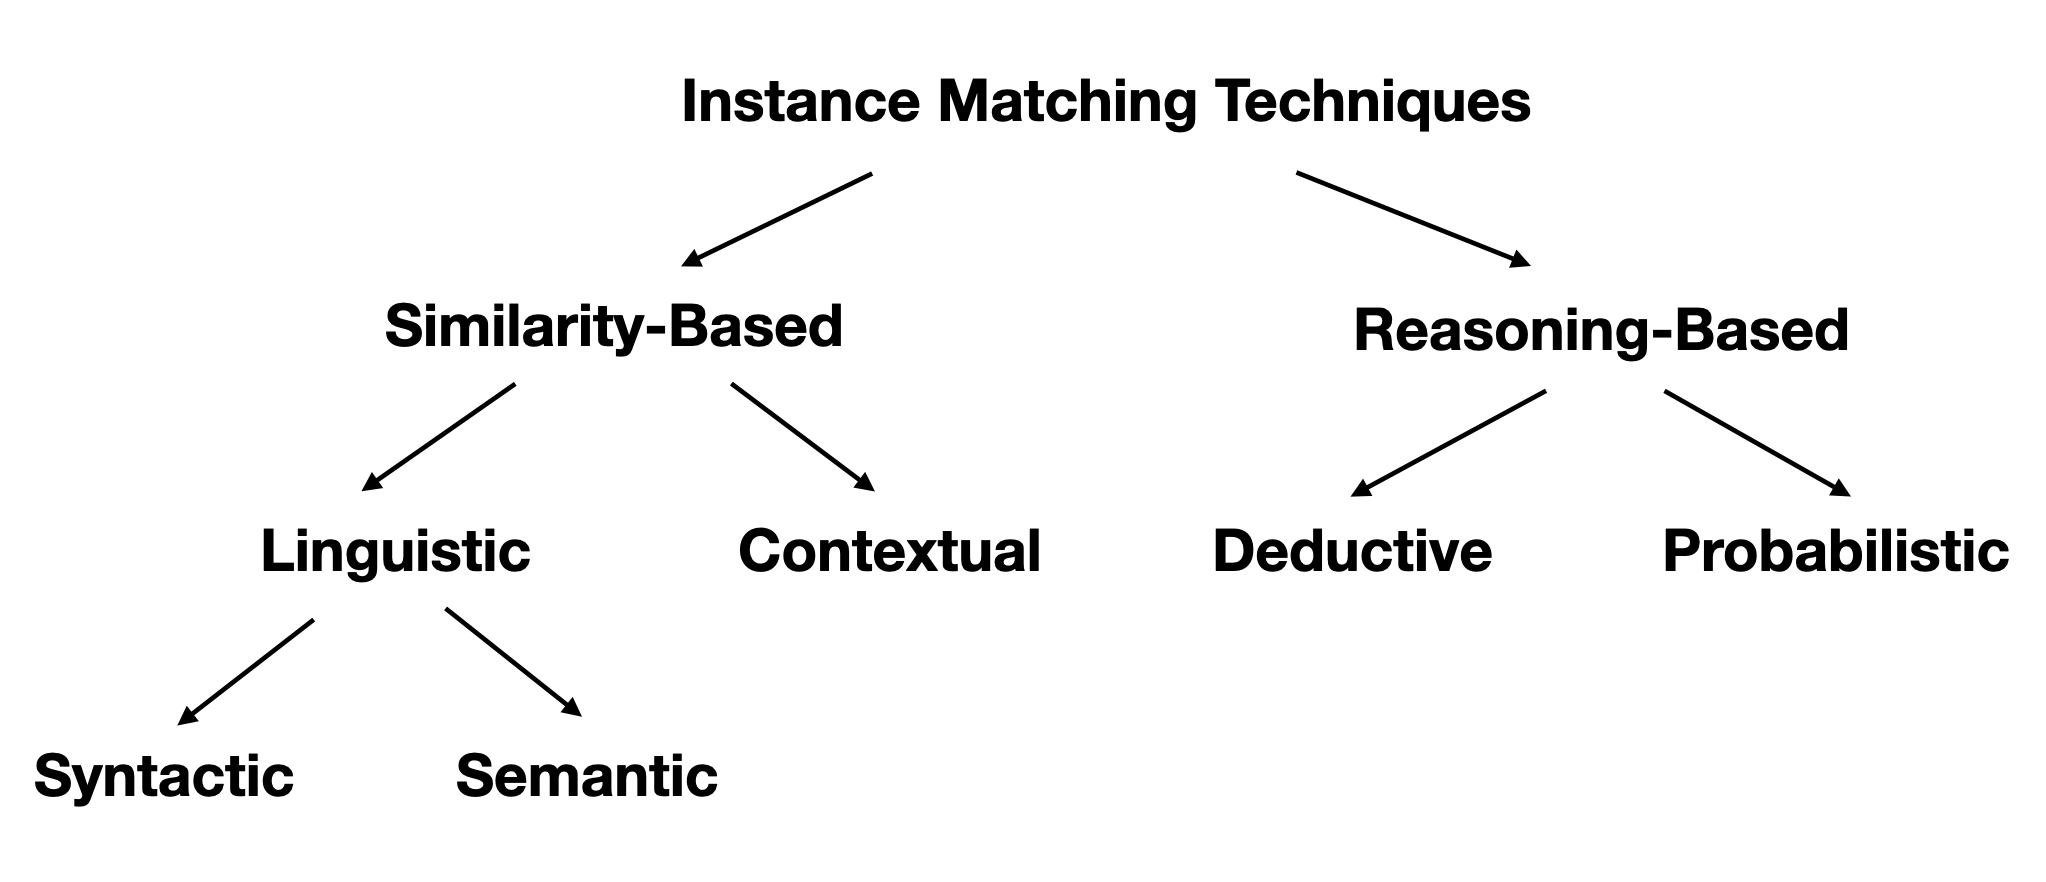
\includegraphics[width=\textwidth]{img/ontology_matching_classification.png}
\caption{Classification of instance matching techniques}
\label{fig:techniques}
\end{figure}

\subsection{Similarity-based}

Similarity-based techniques try to perform a quantitative measurement on the degree of similarity of two entities. Generally speaking, entities are concrete ontological components such as classes, datatypes, properties, and named individuals, and while the main focus is in the context of instance matching, all of them should be considered to facilitate the design of the whole structure. Linguistic similarity and contextual similarity are the two most-used criteria for the measurement \cite{DBLP:conf/ic3k/Nguyen015}.

\subsubsection{Linguistic Similarity}

The linguistic components of an instance are the characteristics related to its string representation. For similarity measurements of strings, syntactic analysis and semantic analysis are the two main approaches.
\\\\
% Syntactic.
The syntactical components of an instance can be the string structure of its name and description, its type constraints, the list of properties it possesses, and so on. Syntactic techniques take advantage of these string structures to discover different kinds and levels of similarities. For example, measures like Edit Distance, Smith-Waterman Distance, and Jaro Distance are based on characters \cite{DBLP:journals/corr/SekerAAM14,DBLP:journals/algorithmica/FaroMP20}, while measures like Cosine Similarity and Q-Gram Distance are based on tokens \cite{DBLP:conf/wea/KobayashiHYS20}. Different weights can be introduced according to the occurrence frequency of the values, so that matches of rare values can receive higher confidence. Further more, phonetic similarities can be discovered with techniques like Soundex \cite{DBLP:journals/corr/BhattiWIHS14} and Metaphone \cite{DBLP:conf/cicling/JordaoR12}, even though their string representations are very different.
\\\\
% Semantic.
Semantic approaches, in contrast, seek to analyse the actual meaning of the entities to be matched, either by informal methods such as looking up dictionaries or thesauri and reading the annotations \cite{DBLP:journals/corr/abs-0907-2209,DBLP:conf/ifip12/LinS08,DBLP:conf/esws/Vennesland15}, or formal methods such as deriving the meaning from semantic definition in other ontologies. Techniques based on this approach first expand the meanings of entities to be matched with synonyms and hyponyms, then evaluate the intersection of their meanings to perform similarity calculations \cite{DBLP:conf/ieaaie/AssiMD19}.

\subsubsection{Contextual Similarity}

Context-based techniques try to match the instances by considering not only their personal attributes, but also how they are defined in their respective \textquotedblleft contexts\textquotedblright, such as object properties and semantic relations with other instances \cite{DBLP:journals/jucs/LinSX12}. The context of an entity can typically be represented as a graph, where entities are denoted by nodes, and properties and semantic relations are denoted by edges. Graph matching algorithms can then be applied to evaluate the topological similarity between the context graphs, therefore determine the similarity between those instances \cite{DBLP:conf/kdd/JehW02}.

\subsection{Reasoning-based}

A fundamental difference between reasoning-based techniques and similarity-based ones is that, in order that reasonings can start, the existence of an initial set of alignments is required as a foundation \cite{DBLP:conf/esws/Meilicke09}. These alignments can be semantic relations already existing between the two ontologies, or manually established by domain experts, or acquired automatically through some similarity-based techniques. Based on these initial alignments, implications of new alignments can be derived by performing various kinds of reasoning tasks. The process goes on iteratively based on the new alignments discovered in the previous iterations, until a time limit or a fixed number of iterations is reached, or no new alignments can be discovered \cite{DBLP:journals/logcom/MeilickeST09}.

\subsubsection{Deductive Reasoning}

Most of the reasoning techniques are considered deductive, as they typically use implication models in the derivation of new candidate alignments. The propositional satisfiability (SAT) model \cite{DBLP:journals/ai/PhamTS08}, for example, treats a candidate alignment between two instances as a propositional formula or implication, whose satisfiability is checked with SAT solvers to determine the correctness of the candidate alignment. Another widely adopted deductive approach is based on the description logic model, in which case existing alignments are used together with rules in the respective ontology such as subsumptions, to exploit and infer new alignments to enrich the initial set \cite{DBLP:phd/ethos/Reul12}.

\subsubsection{Probabilistic Reasoning}

Probabilistic reasoning approaches, on the other hand, try to compute the probability that two instances are identical or similar, by checking whether they have similar set of properties or semantic relations \cite{DBLP:conf/esws/CastanoFLNM08}. Most of them utilise heuristic algorithms \cite{DBLP:conf/jist/NguyenI15}, machine learning techniques or Bayesian networks \cite{DBLP:conf/semweb/SvabS06} for the calculation and propagation of joint probabilities. The interest in techniques that adopt machine learning have been increasing in recent years, however the difficulty in finding a good training dataset is still challenging. Other related techniques based on data analysis and statistical techniques include fuzzy ontologies \cite{DBLP:conf/semweb/TodorovHG13}.


\section{Matching Systems}

A number of matching systems have been proposed in this area, some for general purposes and the other target specific use cases. The list below selects the ones that are most impactful and have distinctive characteristics and gives a brief description of the methodologies they employ.

\begin{spacing}{1.2}
\begin{enumerate}
	\item H-Match: Computes linguistic and contextual similarities and then combine them with weighting schemas to give the final measure of semantic affinity. Common thesauri are used and extended to consider taxonomical or mereological relations.
	\item COMA++: A schema matching tool that utilises string-based techniques, auxiliary thesauri and parallel composition of matchers. Semantically it supports alignment reuse, and structurally it promotes DAG tree matching.
	\item MapOnto: A semi-automated system that constructs complex mapping formulas in Horn clauses. Simple external alignments are taken as part of the input, and structural comparison between the graphical representation of input ontologies are performed.
	\item CtxMatch: Besides the semantic approaches based on strings and WordNet, it exploits description logic reasoners such as Pellet \cite{DBLP:journals/ws/SirinPGKK07} and FaCT \cite{DBLP:conf/cade/TsarkovH06}.
	\item S-Match: Semantic matching is performed based on strings and languages. Entity relations are then translated into propositional formulas using the WordNet dictionary, and resolved with SAT solvers.
	\item Lily: Combines string-based techniques such as Levenshtein Distance and structure-based techniques such as variations of Similarity flooding, to handle large ontologies.
	\item OLA: Compiles the input ontologies into graph structures, then computes string-based, language-based and structure-based similarities. An iterative fixed point algorithm is then performed until no improvements can be discovered.
	\item RiMOM: Uses Bayesian decision theory to automatically discover complex alignments. Taxonomic structure similarities are heuristically discovered and then propagated.
	\item LogMap: Performs lexical indexing using string-based methods and with the help of WordNet. The tree structures of indices are compared, and the matches are repaired using the Dowling-Gallier algorithm based on propositional Horn satisfiability.
	\item PARIS: A probabilistic system that aligns relations, instances and schemas via iterative fixed point computation.
\end{enumerate}
\end{spacing}

It can be discovered that most of the matching systems are schema-based, and tend to focus on specific application domains. Only few of them target the general problem, such as COMA++ and S-Match. Another concern is that most of them handle tree structures while only COMA++ and OLA handle graphs. Further more, only few of them can discover complex correspondences other than the simple one-to-one. And Finally, most of them lack a graphical user interface \cite{euzenat2013d}.

The Ontology Alignment Evaluation Initiative (OAEI)\footnote{\url{http://oaei.ontologymatching.org/}} is a coordinated international initiative to assess strengths and weaknesses of alignment or matching systems, and to compare performance of techniques. It has been organising ontology matching workshops since 2004. Tables \ref{tab:SPIMBENCH_SANDBOX_2020}, \ref{tab:SPIMBENCH_MAINBOX_2020}, \ref{tab:Knowledge_Graph_2020_Overview}, \ref{tab:Knowledge_Graph_2020_Instance_Results} shows the most recent results in 2020 for the SPIMBENCH and Knowledge Graph tracks for the matching systems participated. The reason of considering only these results is that those evaluation tracks focus specifically on instance matching. It can be seen that Lily has achieved excellent precision and recall rate within acceptable time frame, while AML and ATBox outperforms the others in instance matching for Knowledge Graph.

\begin{table}[ht!]
\resizebox{\textwidth}{!}{%
\begin{tabular}{|l|l|l|l|l|l|}
\hline
System          & LogMap-HOBBIT & AgreementMakerLight-Hobbit & Lily\_HOBBIT-2.2 & FTRLIM      & REMiner-1.5 \\ \hline
Fmeasure        & 0.841328413   & 0.864516129                & 0.991708126      & 0.921417565 & 0.998324958 \\ \hline
Precision       & 0.938271605   & 0.834890966                & 0.983552632      & 0.854285714 & 1           \\ \hline
Recall          & 0.762541806   & 0.89632107                 & 1                & 1           & 0.996655518 \\ \hline
timePerformance & 7483          & 6446                       & 2050             & 1525        & 7284        \\ \hline
\end{tabular}%
}
\caption{SPIMBENCH SANDBOX 2020}
\label{tab:SPIMBENCH_SANDBOX_2020}
\end{table}

\begin{table}[ht!]
\resizebox{\textwidth}{!}{%
\begin{tabular}{|l|l|l|l|l|l|}
\hline
System          & LogMap-HOBBIT & AgreementMakerLight-Hobbit & Lily\_HOBBIT-2.2 & FTRLIM      & REMiner-1.5 \\ \hline
Fmeasure        & 0.785635764   & 0.860457622                & 0.995388669      & 0.921478766 & 0.997681351 \\ \hline
Precision       & 0.880131363   & 0.838567839                & 0.990819672      & 0.85584563  & 0.99867374  \\ \hline
Recall          & 0.709463931   & 0.883520847                & 1                & 0.99801456  & 0.996690933 \\ \hline
timePerformance & 26782         & 38772                      & 3899             & 2247        & 33966       \\ \hline
\end{tabular}%
}
\caption{SPIMBENCH MAINBOX 2020}
\label{tab:SPIMBENCH_MAINBOX_2020}
\end{table}

\begin{table}[ht!]
\resizebox{\textwidth}{!}{%
\begin{tabular}{|l|l|l|l|l|l|l|l|l|l|l|l|l|l|l|l|l|l|l|}
\hline
\multicolumn{1}{|c|}{\textbf{}}       & \multicolumn{1}{c|}{\textbf{}}     & \multicolumn{4}{c|}{\textbf{class}}                                                                                                                       & \multicolumn{4}{c|}{\textbf{property}}                                                                                                             & \multicolumn{4}{c|}{\textbf{instance}}                                                                                                             & \multicolumn{4}{c|}{\textbf{overall}}                                                                                                              &                                    \\ \hline
\multicolumn{1}{|c|}{\textbf{System}} & \multicolumn{1}{c|}{\textbf{Time}} & \multicolumn{1}{c|}{\textbf{\#testcases}} & \multicolumn{1}{c|}{\textbf{Size}} & \multicolumn{1}{c|}{\textbf{Prec.}} & \multicolumn{1}{c|}{\textbf{F-m.}} & \multicolumn{1}{c|}{\textbf{Rec.}} & \multicolumn{1}{c|}{\textbf{Size}} & \multicolumn{1}{c|}{\textbf{Prec.}} & \multicolumn{1}{c|}{\textbf{F-m.}} & \multicolumn{1}{c|}{\textbf{Rec.}} & \multicolumn{1}{c|}{\textbf{Size}} & \multicolumn{1}{c|}{\textbf{Prec.}} & \multicolumn{1}{c|}{\textbf{F-m.}} & \multicolumn{1}{c|}{\textbf{Rec.}} & \multicolumn{1}{c|}{\textbf{Size}} & \multicolumn{1}{c|}{\textbf{Prec.}} & \multicolumn{1}{c|}{\textbf{F-m.}} & \multicolumn{1}{c|}{\textbf{Rec.}} \\ \hline
ALOD2Vec                              & 0:13:24                            & 5                                         & 20.0                               & 1.00 (1.00)                         & 0.80 (0.80)                        & 0.67 (0.67)                        & 76.8                               & 0.94 (0.94)                         & 0.95 (0.95)                        & 0.97 (0.97)                        & 4893.8                             & 0.91 (0.91)                         & 0.87 (0.87)                        & 0.83 (0.83)                        & 4990.6                             & 0.91 (0.91)                         & 0.87 (0.87)                        & 0.83 (0.83)                        \\ \hline
AML                                   & 0:50:55                            & 5                                         & 23.6                               & 0.98 (0.98)                         & 0.89 (0.89)                        & 0.81 (0.81)                        & 48.4                               & 0.92 (0.92)                         & 0.70 (0.70)                        & 0.57 (0.57)                        & 6802.8                             & 0.90 (0.90)                         & 0.85 (0.85)                        & 0.80 (0.80)                        & 6874.8                             & 0.90 (0.90)                         & 0.85 (0.85)                        & 0.80 (0.80)                        \\ \hline
ATBox                                 & 0:16:22                            & 5                                         & 25.6                               & 0.97 (0.97)                         & 0.87 (0.87)                        & 0.79 (0.79)                        & 78.8                               & 0.97 (0.97)                         & 0.96 (0.96)                        & 0.95 (0.95)                        & 4858.8                             & 0.89 (0.89)                         & 0.84 (0.84)                        & 0.80 (0.80)                        & 4963.2                             & 0.89 (0.89)                         & 0.85 (0.85)                        & 0.81 (0.81)                        \\ \hline
baselineAltLabel                      & 0:10:57                            & 5                                         & 16.4                               & 1.00 (1.00)                         & 0.74 (0.74)                        & 0.59 (0.59)                        & 47.8                               & 0.99 (0.99)                         & 0.79 (0.79)                        & 0.66 (0.66)                        & 4674.8                             & 0.89 (0.89)                         & 0.84 (0.84)                        & 0.80 (0.80)                        & 4739.0                             & 0.89 (0.89)                         & 0.84 (0.84)                        & 0.80 (0.80)                        \\ \hline
baselineLabel                         & 0:10:44                            & 5                                         & 16.4                               & 1.00 (1.00)                         & 0.74 (0.74)                        & 0.59 (0.59)                        & 47.8                               & 0.99 (0.99)                         & 0.79 (0.79)                        & 0.66 (0.66)                        & 3641.8                             & 0.95 (0.95)                         & 0.81 (0.81)                        & 0.71 (0.71)                        & 3706.0                             & 0.95 (0.95)                         & 0.81 (0.81)                        & 0.71 (0.71)                        \\ \hline
DESKMatcher                           & 0:13:54                            & 5                                         & 91.4                               & 0.76 (0.76)                         & 0.71 (0.71)                        & 0.66 (0.66)                        & 0.0                                & 0.00 (0.00)                         & 0.00 (0.00)                        & 0.00 (0.00)                        & 3820.6                             & 0.94 (0.94)                         & 0.82 (0.82)                        & 0.74 (0.74)                        & 3912.0                             & 0.93 (0.93)                         & 0.81 (0.81)                        & 0.72 (0.72)                        \\ \hline
LogMap                                & 2:55:14                            & 5                                         & 24.0                               & 0.95 (0.95)                         & 0.84 (0.84)                        & 0.76 (0.76)                        & 0.0                                & 0.00 (0.00)                         & 0.00 (0.00)                        & 0.00 (0.00)                        & 29190.4                            & 0.40 (0.40)                         & 0.54 (0.54)                        & 0.86 (0.86)                        & 29214.4                            & 0.40 (0.40)                         & 0.54 (0.54)                        & 0.84 (0.84)                        \\ \hline
LogMapBio                             & 4:35:29                            & 5                                         & 24.0                               & 0.95 (0.95)                         & 0.84 (0.84)                        & 0.76 (0.76)                        & 0.0                                & 0.00 (0.00)                         & 0.00 (0.00)                        & 0.00 (0.00)                        & 0.0                                & 0.00 (0.00)                         & 0.00 (0.00)                        & 0.00 (0.00)                        & 24.0                               & 0.95 (0.95)                         & 0.01 (0.01)                        & 0.00 (0.00)                        \\ \hline
LogMapIM                              & 2:49:34                            & 5                                         & 0.0                                & 0.00 (0.00)                         & 0.00 (0.00)                        & 0.00 (0.00)                        & 0.0                                & 0.00 (0.00)                         & 0.00 (0.00)                        & 0.00 (0.00)                        & 29190.4                            & 0.40 (0.40)                         & 0.54 (0.54)                        & 0.86 (0.86)                        & 29190.4                            & 0.40 (0.40)                         & 0.54 (0.54)                        & 0.84 (0.84)                        \\ \hline
LogMapKG                              & 2:47:51                            & 5                                         & 24.0                               & 0.95 (0.95)                         & 0.84 (0.84)                        & 0.76 (0.76)                        & 0.0                                & 0.00 (0.00)                         & 0.00 (0.00)                        & 0.00 (0.00)                        & 29190.4                            & 0.40 (0.40)                         & 0.54 (0.54)                        & 0.86 (0.86)                        & 29214.4                            & 0.40 (0.40)                         & 0.54 (0.54)                        & 0.84 (0.84)                        \\ \hline
LogMapLt                              & 0:07:19                            & 4                                         & 23.0                               & 0.80 (1.00)                         & 0.56 (0.70)                        & 0.43 (0.54)                        & 0.0                                & 0.00 (0.00)                         & 0.00 (0.00)                        & 0.00 (0.00)                        & 6653.8                             & 0.73 (0.91)                         & 0.67 (0.84)                        & 0.62 (0.78)                        & 6676.8                             & 0.73 (0.92)                         & 0.66 (0.83)                        & 0.61 (0.76)                        \\ \hline
Wiktionary                            & 0:30:12                            & 5                                         & 22.4                               & 1.00 (1.00)                         & 0.80 (0.80)                        & 0.67 (0.67)                        & 80.0                               & 0.94 (0.94)                         & 0.95 (0.95)                        & 0.97 (0.97)                        & 4893.8                             & 0.91 (0.91)                         & 0.87 (0.87)                        & 0.83 (0.83)                        & 4996.2                             & 0.91 (0.91)                         & 0.87 (0.87)                        & 0.83 (0.83)                        \\ \hline
\end{tabular}%
}
\caption{Knowledge Graph 2020 Overview}
\label{tab:Knowledge_Graph_2020_Overview}
\end{table}

\begin{table}[ht!]
\resizebox{\textwidth}{!}{%
\begin{tabular}{|l|l|l|l|l|l|l|l|l|l|l|l|l|l|l|l|l|l|l|l|l|}
\hline
\multicolumn{4}{|c|}{\textbf{marvelcinematicuniverse-marvel}}                                                                                   & \multicolumn{4}{c|}{\textbf{memoryalpha-memorybeta}}                                                                                               & \multicolumn{4}{c|}{\textbf{memoryalpha-stexpanded}}                                                                                               & \multicolumn{4}{c|}{\textbf{starwars-swg}}                                                                                                         & \multicolumn{4}{c|}{\textbf{starwars-swtor}}                                                                                                       &                                    \\ \hline
\multicolumn{1}{|c|}{\textbf{}} & \multicolumn{1}{c|}{\textbf{Size}} & \multicolumn{1}{c|}{\textbf{Prec.}} & \multicolumn{1}{c|}{\textbf{F-m.}} & \multicolumn{1}{c|}{\textbf{Rec.}} & \multicolumn{1}{c|}{\textbf{Size}} & \multicolumn{1}{c|}{\textbf{Prec.}} & \multicolumn{1}{c|}{\textbf{F-m.}} & \multicolumn{1}{c|}{\textbf{Rec.}} & \multicolumn{1}{c|}{\textbf{Size}} & \multicolumn{1}{c|}{\textbf{Prec.}} & \multicolumn{1}{c|}{\textbf{F-m.}} & \multicolumn{1}{c|}{\textbf{Rec.}} & \multicolumn{1}{c|}{\textbf{Size}} & \multicolumn{1}{c|}{\textbf{Prec.}} & \multicolumn{1}{c|}{\textbf{F-m.}} & \multicolumn{1}{c|}{\textbf{Rec.}} & \multicolumn{1}{c|}{\textbf{Size}} & \multicolumn{1}{c|}{\textbf{Prec.}} & \multicolumn{1}{c|}{\textbf{F-m.}} & \multicolumn{1}{c|}{\textbf{Rec.}} \\ \hline
ALOD2Vec                        & 3065                               & 0.86                                & 0.76                               & 0.68                               & 13325                              & 0.92                                & 0.91                               & 0.90                               & 3285                               & 0.92                                & 0.93                               & 0.93                               & 2118                               & 0.92                                & 0.82                               & 0.75                               & 2676                               & 0.92                                & 0.92                               & 0.91                               \\ \hline
AML                             & 4670                               & 0.85                                & 0.68                               & 0.56                               & 18319                              & 0.91                                & 0.89                               & 0.87                               & 3699                               & 0.93                                & 0.93                               & 0.93                               & 3491                               & 0.90                                & 0.81                               & 0.75                               & 3835                               & 0.93                                & 0.92                               & 0.90                               \\ \hline
ATBox                           & 3483                               & 0.66                                & 0.58                               & 0.52                               & 12860                              & 0.96                                & 0.93                               & 0.91                               & 3162                               & 0.96                                & 0.94                               & 0.92                               & 2170                               & 0.93                                & 0.83                               & 0.76                               & 2619                               & 0.94                                & 0.92                               & 0.91                               \\ \hline
baselineAltLabel                & 2559                               & 0.86                                & 0.76                               & 0.68                               & 13454                              & 0.88                                & 0.89                               & 0.89                               & 3165                               & 0.88                                & 0.90                               & 0.93                               & 1661                               & 0.92                                & 0.74                               & 0.62                               & 2535                               & 0.92                                & 0.91                               & 0.90                               \\ \hline
baselineLabel                   & 1864                               & 0.90                                & 0.69                               & 0.56                               & 10492                              & 0.95                                & 0.85                               & 0.77                               & 2517                               & 0.98                                & 0.91                               & 0.84                               & 1194                               & 0.95                                & 0.67                               & 0.52                               & 2142                               & 0.95                                & 0.89                               & 0.84                               \\ \hline
DESKMatcher                     & 1898                               & 0.89                                & 0.69                               & 0.56                               & 10831                              & 0.94                                & 0.85                               & 0.78                               & 2557                               & 0.98                                & 0.91                               & 0.84                               & 1522                               & 0.93                                & 0.76                               & 0.64                               & 2295                               & 0.94                                & 0.90                               & 0.86                               \\ \hline
LogMap                          & 41070                              & 0.24                                & 0.35                               & 0.71                               & 54499                              & 0.43                                & 0.58                               & 0.87                               & 15529                              & 0.47                                & 0.63                               & 0.94                               & 15323                              & 0.58                                & 0.68                               & 0.82                               & 19531                              & 0.27                                & 0.42                               & 0.96                               \\ \hline
LogMapBio                       & 0                                  & 0.00                                & 0.00                               & 0.00                               & 0                                  & 0.00                                & 0.00                               & 0.00                               & 0                                  & 0.00                                & 0.00                               & 0.00                               & 0                                  & 0.00                                & 0.00                               & 0.00                               & 0                                  & 0.00                                & 0.00                               & 0.00                               \\ \hline
LogMapIM                        & 41070                              & 0.24                                & 0.35                               & 0.71                               & 54499                              & 0.43                                & 0.58                               & 0.87                               & 15529                              & 0.47                                & 0.63                               & 0.94                               & 15323                              & 0.58                                & 0.68                               & 0.82                               & 19531                              & 0.27                                & 0.42                               & 0.96                               \\ \hline
LogMapKG                        & 41070                              & 0.24                                & 0.35                               & 0.71                               & 54499                              & 0.43                                & 0.58                               & 0.87                               & 15529                              & 0.47                                & 0.63                               & 0.94                               & 15323                              & 0.58                                & 0.68                               & 0.82                               & 19531                              & 0.27                                & 0.42                               & 0.96                               \\ \hline
LogMapLt                        & 0                                  & 0.00                                & 0.00                               & 0.00                               & 16665                              & 0.90                                & 0.83                               & 0.77                               & 3550                               & 0.94                                & 0.89                               & 0.84                               & 2795                               & 0.91                                & 0.75                               & 0.63                               & 3605                               & 0.91                                & 0.89                               & 0.87                               \\ \hline
Wiktionary                      & 3065                               & 0.86                                & 0.76                               & 0.68                               & 13327                              & 0.92                                & 0.91                               & 0.90                               & 3283                               & 0.92                                & 0.92                               & 0.93                               & 2118                               & 0.92                                & 0.82                               & 0.75                               & 2676                               & 0.92                                & 0.92                               & 0.91                               \\ \hline
\end{tabular}%
}
\caption{Knowledge Graph 2020 Instance Results}
\label{tab:Knowledge_Graph_2020_Instance_Results}
\end{table}

\section{System Development}

Various tools, evaluation frameworks and APIs are provided by the ontology matching industry, and can be utilised in the development of matching systems. An introduction to the ones related to this project is given below.

\subsection{Tools}

Protégé\footnote{\url{https://protege.stanford.edu}} \cite{DBLP:journals/aimatters/Musen15} is an open-source ontology editor with a friendly user interface and lots of plug-ins such as OWL/RDF parsers or description logic reasoners. Besides basic editing over ontologies, functionalities such as converting axioms and reasoning about inconsistencies can be achieved. It has been used for manipulating the toy datasets and visualising the class hierarchies of OWL 2 ontologies, and will be used for general purpose ontology editing in the later stages.
\\\\
For the visualisation of alignments, tools such as HOMER and AlViz \cite{DBLP:conf/iv/LanzenbergerS06} exist. Although visualising the alignments is not within the objectives of the project, it is beneficial to use such tools to check the results of smaller-scaled matching tasks.

\subsection{Evaluation Frameworks}

OAEI provides two evaluation frameworks, SEALS\footnote{\url{http://oaei.ontologymatching.org/2020/seals/index.html}} and HOBBIT\footnote{\url{http://oaei.ontologymatching.org/2020/hobbit/index.html}}, that can be adopted for the running of different benchmark tracks. A total of 12 evaluation tracks are provided in the two benchmark frameworks: Anatomy (SEALS), Conference (SEALS), Multifarm (SEALS), Complex (SEALS), Interactive matching (SEALS), Largebio (SEALS, HOBBIT), Phenotype (SEALS), Biodiversity and Ecology (SEALS), SPIMBENCH (HOBBIT), Link Discovery (HOBBIT), GeoLink Cruise (SEALS) and Knowledge Graph (SEALS, HOBBIT). While most of them focus on the evaluation of schema matching, three of them, namely SPIMBENCH, Link Discovery, and Knowledge Graph, are suitable for the evaluation of instance matching.
\\\\
SPIMBENCH seeks to determine whether two instances describe the same Creative Work, where value-based, structure-based, and semantics-aware transformations are made to the original dataset to produce the new dataset to be matched with. This is ideal for the evaluation of this project. Link Discovery focuses more on spacial data, and Knowledge Graph aims at matching both schema and instances. These two can be used to complement the evaluation result to be more general. As all three of these are provided within the HOBBIT framework, the implementation will be wrapped in HOBBIT using the HOBBIT Java SDK\footnote{\url{https://github.com/hobbit-project/java-sdk}}.

\subsection{APIs}

The OWL API\footnote{\url{https://github.com/owlcs/owlapi}} can be used for creating, manipulating and serialising OWL ontologies, and its latest version 5.1.17 is OWL 2 compatible. As the implementation will target the matching of OWL 2 ontologies only, the OWL API is the absolute necessity throughout the implementation stages.
\\\\
For the most powerful description logic reasoners such as HermiT \cite{DBLP:journals/jar/GlimmHMSW14} and FaCT++ \cite{DBLP:conf/cade/TsarkovH06}, they can not only be used as plug-ins for Protégé, but also be used as Java APIs. This means that specific functionalities can be invoked from the code instead of having to run the whole reasoner. These reasoner APIs are crucial in the development stage of reasoning-based techniques, and also in the evaluation stage for reasoning about the matched instances after the majority of the implementation tasks have finished.
\\\\
The Alignment API\footnote{\url{http://alignapi.gforge.inria.fr}} can be used for generating and sharing ontology alignments that are compatible with the evaluation frameworks. As the implementation will be wrapped in HOBBIT to perform local tests, it is necessary to use the Alignment API so that matching results are comparable by the framework.
\\\\
Since the ultimate aim of this project is to support the tasks of data integration, the querying of the integrated dataset should be implemented. This can be done with the help of SPARQL-Generate API\footnote{\url{https://github.com/sparql-generate}}, which provides a standard mechanism to search for semantic contents.


\chapter{Methodology}

This chapter contains a comprehensive description of the design of the proposed matching system, demonstrates how it addresses the problem, and justifies the design with the support of evaluation results.

The workflow of a typical ontology matching methodology is given in Figure \ref{fig:methodology}. The central part, being "selecting and composing matchers", is the stage that should be put most effort on.

\begin{figure}[ht]
\begin{center}
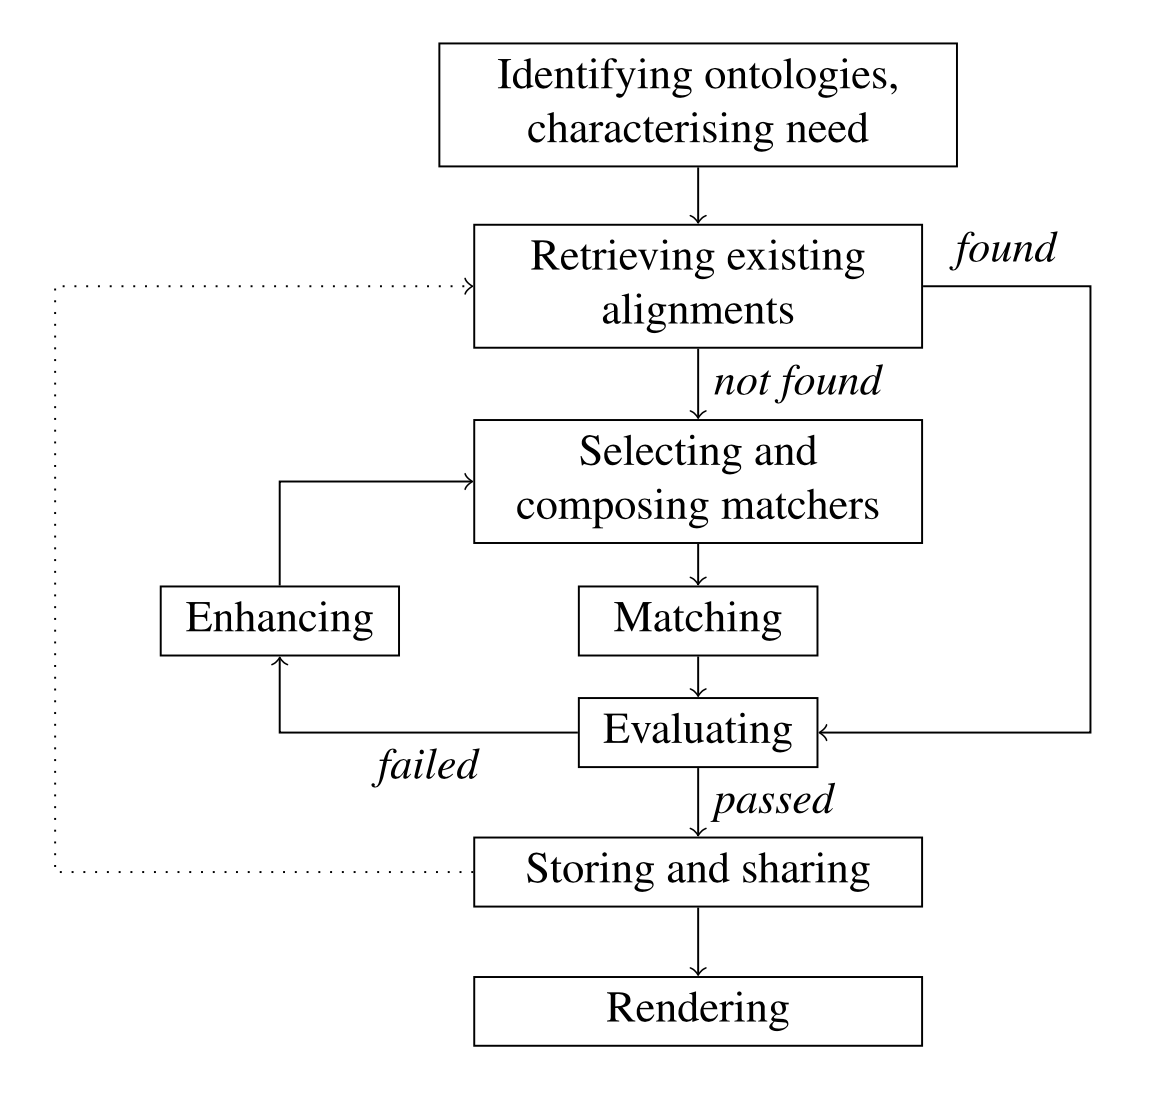
\includegraphics[width=0.4\textwidth]{img/methodology.png}
\caption{The matching methodology workflow}
\label{fig:methodology}
\end{center}
\end{figure}

According to the structures of existing popular systems and the evaluation results provided in the previous chapter, the structures of three systems, namely Lily, LogMap and PARIS, are the ones decided to be focused on. Lily has shown excellent performance in the SPIMBENCH instance matching tracks, with not only high precision, F-measure and recall rate, but also a reasonable time efficiency. LogMap was designed to be able to deal with large-scaled ontologies in general purposes, which suits the need of matching enormous instances in data integration. PARIS, being a probability-based system, deals with not only classes and instances, but also tries to align relations. This can be used as an ideal start of the project, the fundamental aim of which being investigating the aid of matching object relations in instance matching. Based on the common points of their structures, the following design selects methodological components to be used and propose a basic structure of integrating them.

\begin{spacing}{1.2}
\begin{enumerate}
	\item The components in the input ontologies, including not only classes and instances, but also object properties, data properties, values and relation roles between different instances, are interpreted as strings.
	\item String-based techniques such as Levenshtein Distance and lexical indexing are then used to discover their syntactical similarities.
	\item Public general-purpose dictionaries such as WordNet may be considered for the semantic evaluation of the strings.
	\item A preliminary match between the corresponding entities is performed, where the alignments with highest confidence are kept.
	\item Based on the existing matches available, description logic reasoners are exploited for the inference of nontrivial relations.
	\item Structure-based techniques such as similarity flooding are adopted to determine the matching instances by checking the similarity between their adjacently related instances.
	\item Description logic reasoners are used for a systematic discovery of inconsistencies based on the matching instances and logical relations. Pruning will be carried out if inconsistencies are identified.
\end{enumerate}
\end{spacing}

It should be noted that although these are the proposed algorithmic components are currently decided as suitable for the general purpose instance matching, the selection and combinational order of them is subject to changes and required more detailed design. Further knowledge about the linkage of those components in existing systems should be acquired, which is the current and next stage of this project.

\chapter{Implementation}

% This chapter contains a comprehensive description of the implementation of your software, including the language(s) and platform chosen, problems encountered, any changes made to the design as a result of the implementation, etc.

% Explaining how your software was tested (using different datasets or in different environments), statistical evaluation of performance, results of user evaluation questionnaires, etc.

For the implementation of the proposed instance matching system, Java will be used as the primary programming language, as the supplementary APIs and evaluation initiatives use Java officially. This chapter introduces some core Java classes and functions from the APIs and SDKs that will be used in the implementation.

\section{Development}

\subsection{OWL API}

In order to perform basic manipulation over the entities in OWL 2 ontologies, the \\
\texttt{org.semanticweb.owlapi.model} package should be utilised. Specifically, classes like \texttt{AddAxiom}, \texttt{AddImport}, \texttt{AddOntologyAnnotation} and their corresponding removers are the fundamental operations that will be used along.
\\\\
Parser and renderer classes are available for various OWL 2 syntaxes, including the OWL/XML, RDF/XML, DL, functional, Manchester and Turtle, in their respective packages. The \texttt{parse} and \texttt{render} function can be used to read from one syntax and then write into another. These can be useful when another desired software tool or API have support issues with specific syntaxes.
\\\\
Classes inside the package \texttt{org.semanticweb.owlapi.profiles} can be used to check whether an input ontology falls into a certain OWL 2 profile. This helps in analysing the reasonability and decidability for tasks provided in the evaluation framework.
\\\\
The \texttt{org.semanticweb.owlapi.vocab} package contains \texttt{Enum} classes, such as \\
\texttt{BuiltInVocabulary}, \texttt{Namespaces} and \texttt{OWL2Datatype}, that enumerate various kinds of OWL 2 vocabularies. These are useful for custom construction and interpretation of expressions.
\\\\
While the implementation does not build a reasoner for itself, the package \\
\texttt{org.semanticweb.owlapi.reasoner} is required for the reasoner APIs to be based on.

\subsection{Reasoner API}

While different reasoners have different usages, their core components and functionalities are similar. Take the HermiT reasoner for example, the \texttt{org.semanticweb.HermiT.model} package contains class definitions for logical models such as equality, inequality, role, inverse role, atomic concept, atomic role, and so on, while the \\
\texttt{org.semanticweb.HermiT.structural} package contains classes that manages the structure of built-in properties and axioms.

\subsection{Alignment API}

For the basic use of Alignment API, the package \texttt{fr.inrialpes.exmo.align.parser} is sufficient for the parsing of alignment syntax. The API also provides a WordNet-based implementation besides the basic implementation.

\subsection{SPARQL-Generate API}

The \texttt{fr.mines\_stetienne.ci.sparql\_generate.query} package in SPARQL-Generate API contains the model for SPARQL queries, which is used for query construction. The package \texttt{fr.mines\_stetienne.ci.sparql\_generate.engine} can then be used to execute the query using one of the \texttt{exec} methods in its classes.

\section{Evaluation}

In order to evaluate the instance matching results, the implementation needs to be wrapped in the HOBBIT evaluation framework \cite{}. HOBBIT has provided a library called the HOBBIT Java SDK to simplify the wrapping as well as local testing with supported data. In order to use the SDK, the Maven environment should be set up properly according to \url{https://hobbit-project.github.io/java_components}. Then the components of a benchmark should be made to implement the \texttt{org.hobbit.core.components.Component} interface. The details of system adapter development and benchmark components should be investigated into details.


\chapter{Progress and Reflection}

This chapter illustrates various aspects reside in the management of the project, including a revision of the original workplan, a description of the working methodology, resource management details and contingency measures. A personal reflection to the project during its first half is also presented. 

\section{Project Management}
% Covering the tasks as a part of your work plan and progress as well as how time and resources are managed.

\subsection{Revision of Workplan}
% Revision of workplan.
Figure \ref{fig:Gantt_old} shows the proposed workplan of the project designed at the beginning stage. Generally speaking, the progress of the project has been satisfying, as all the phases involving literature review and systematic learning have been completed on time. One task was shelved and left behind schedule, however, namely the delivery of an ontology matching framework, which was supposed to come along with the interim report. There are two primary contributing factors to the making of this decision. Firstly, the workload in studying existing ontology matching techniques was underestimated, making the expectation of designing the framework simultaneously with the learning process unrealistic. Secondly, time allocation was inevitably tilted to the investigation of instance matching strategies, as they are inseparable from the general ontology matching framework. This was considered better for the selection of suitable framework components after some investigation into ontology matching, and was hence given higher priority.
\\\\
In order to reflect the above changes, a revised workplan was designed and presented in figure \ref{fig:Gantt_new}. The project is currently at the milestone of Interim Report, and the progress until present is demonstrated in the previous stages. Due to the effect of exam preparation, implementation tasks before the exams are only preliminary, while the major development tasks are put in the winter vacation. This is sensible because coding and debugging can take a large amount of time. The adjustment of instance matching algorithm is now side by side with testing and evaluation, with the validation of design carried all along the way. In the case of unexpected obstacles or potential risks such as increased academic workload during the spring semester, the adjustment phase can shrink to buffer the impact on the overall workplan. The workload of writing the final dissertation is spread over a longer timespan, as it was discovered that writing usually takes longer than expected.

\begin{figure}[ht]
\begin{subfigure}[ht]{\textwidth}
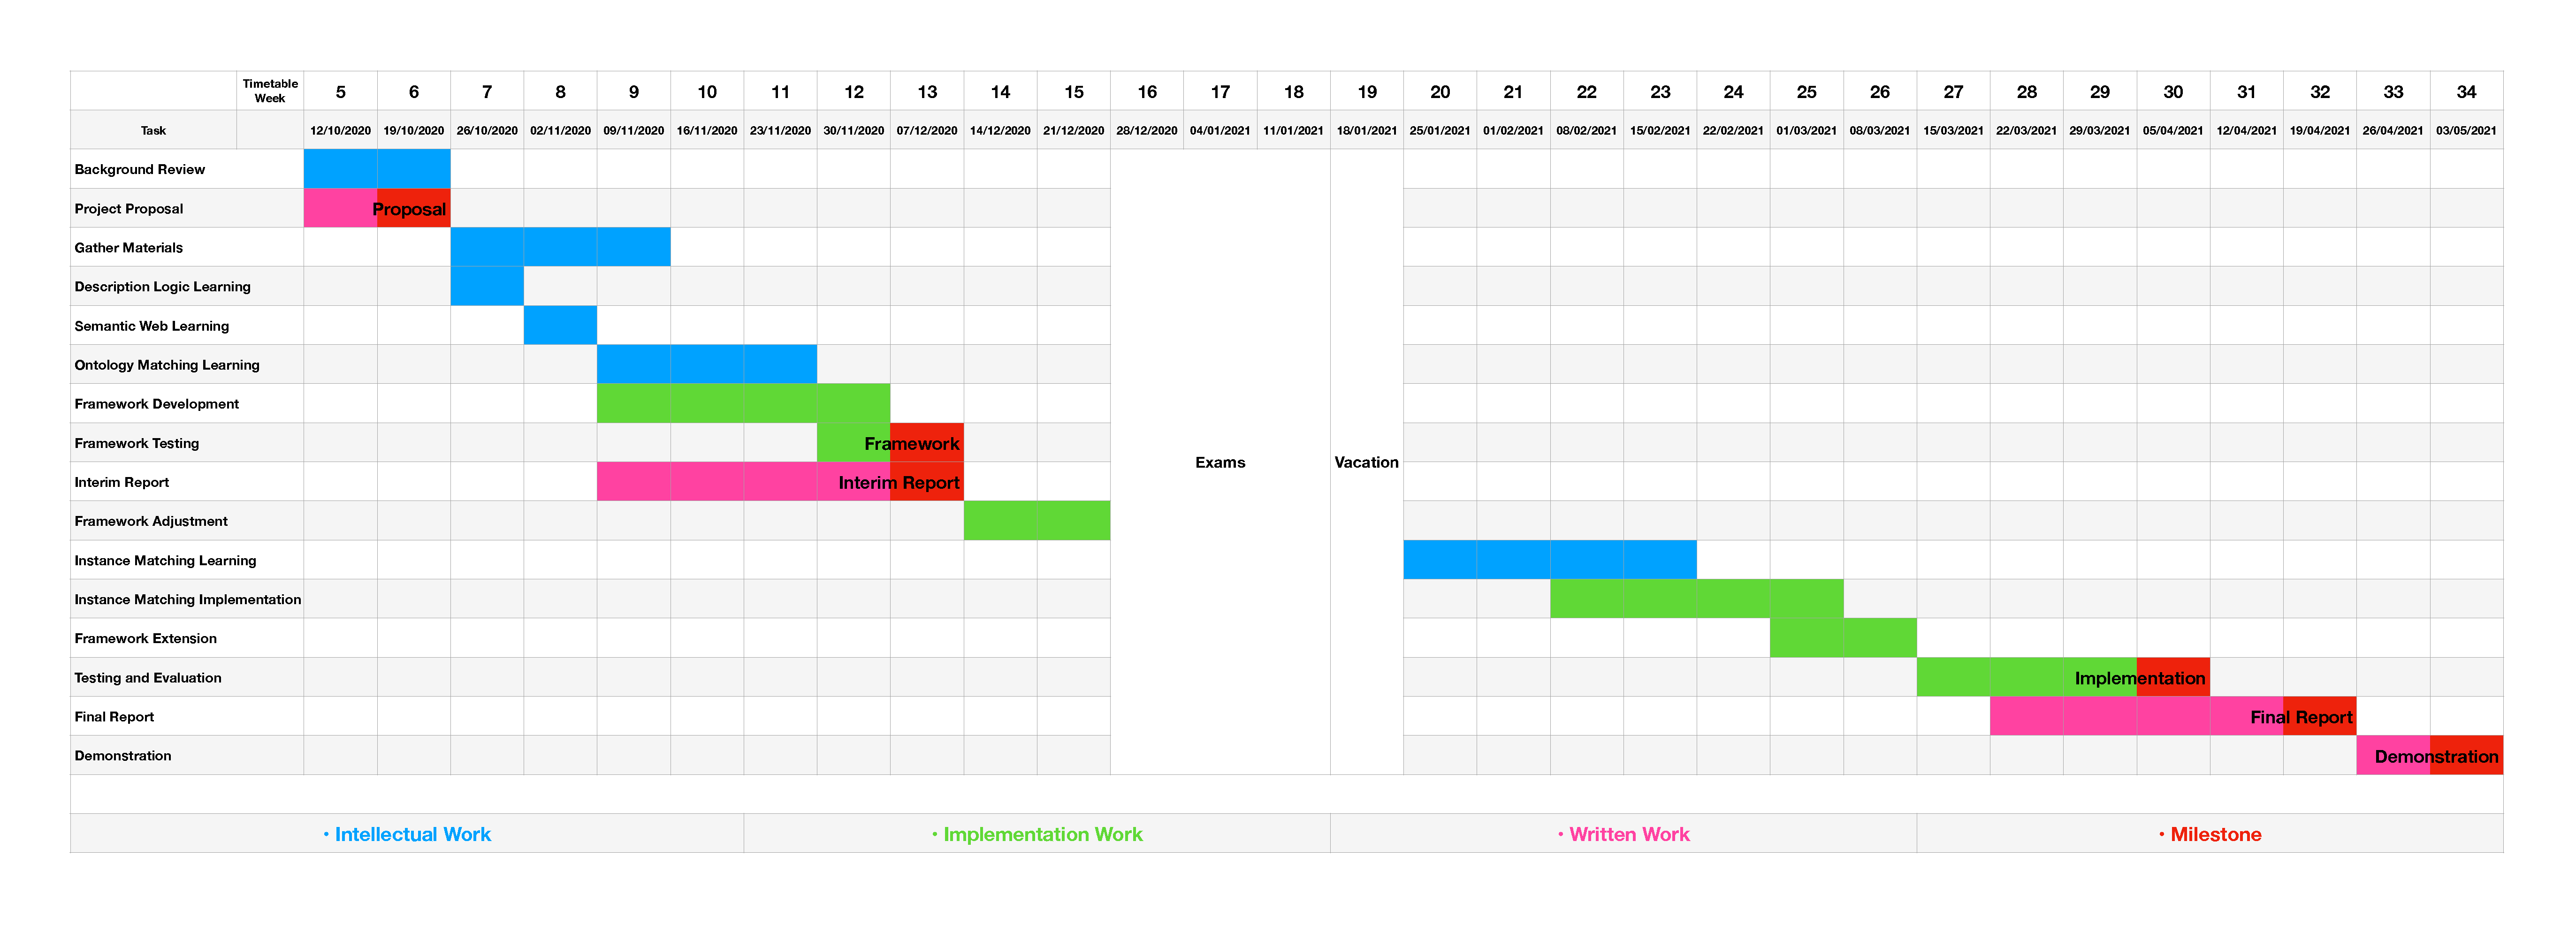
\includegraphics[width=\textwidth]{img/Gantt_old.pdf}
\caption{Original workplan}
\label{fig:Gantt_old}
\end{subfigure}
\begin{subfigure}[ht]{\textwidth}
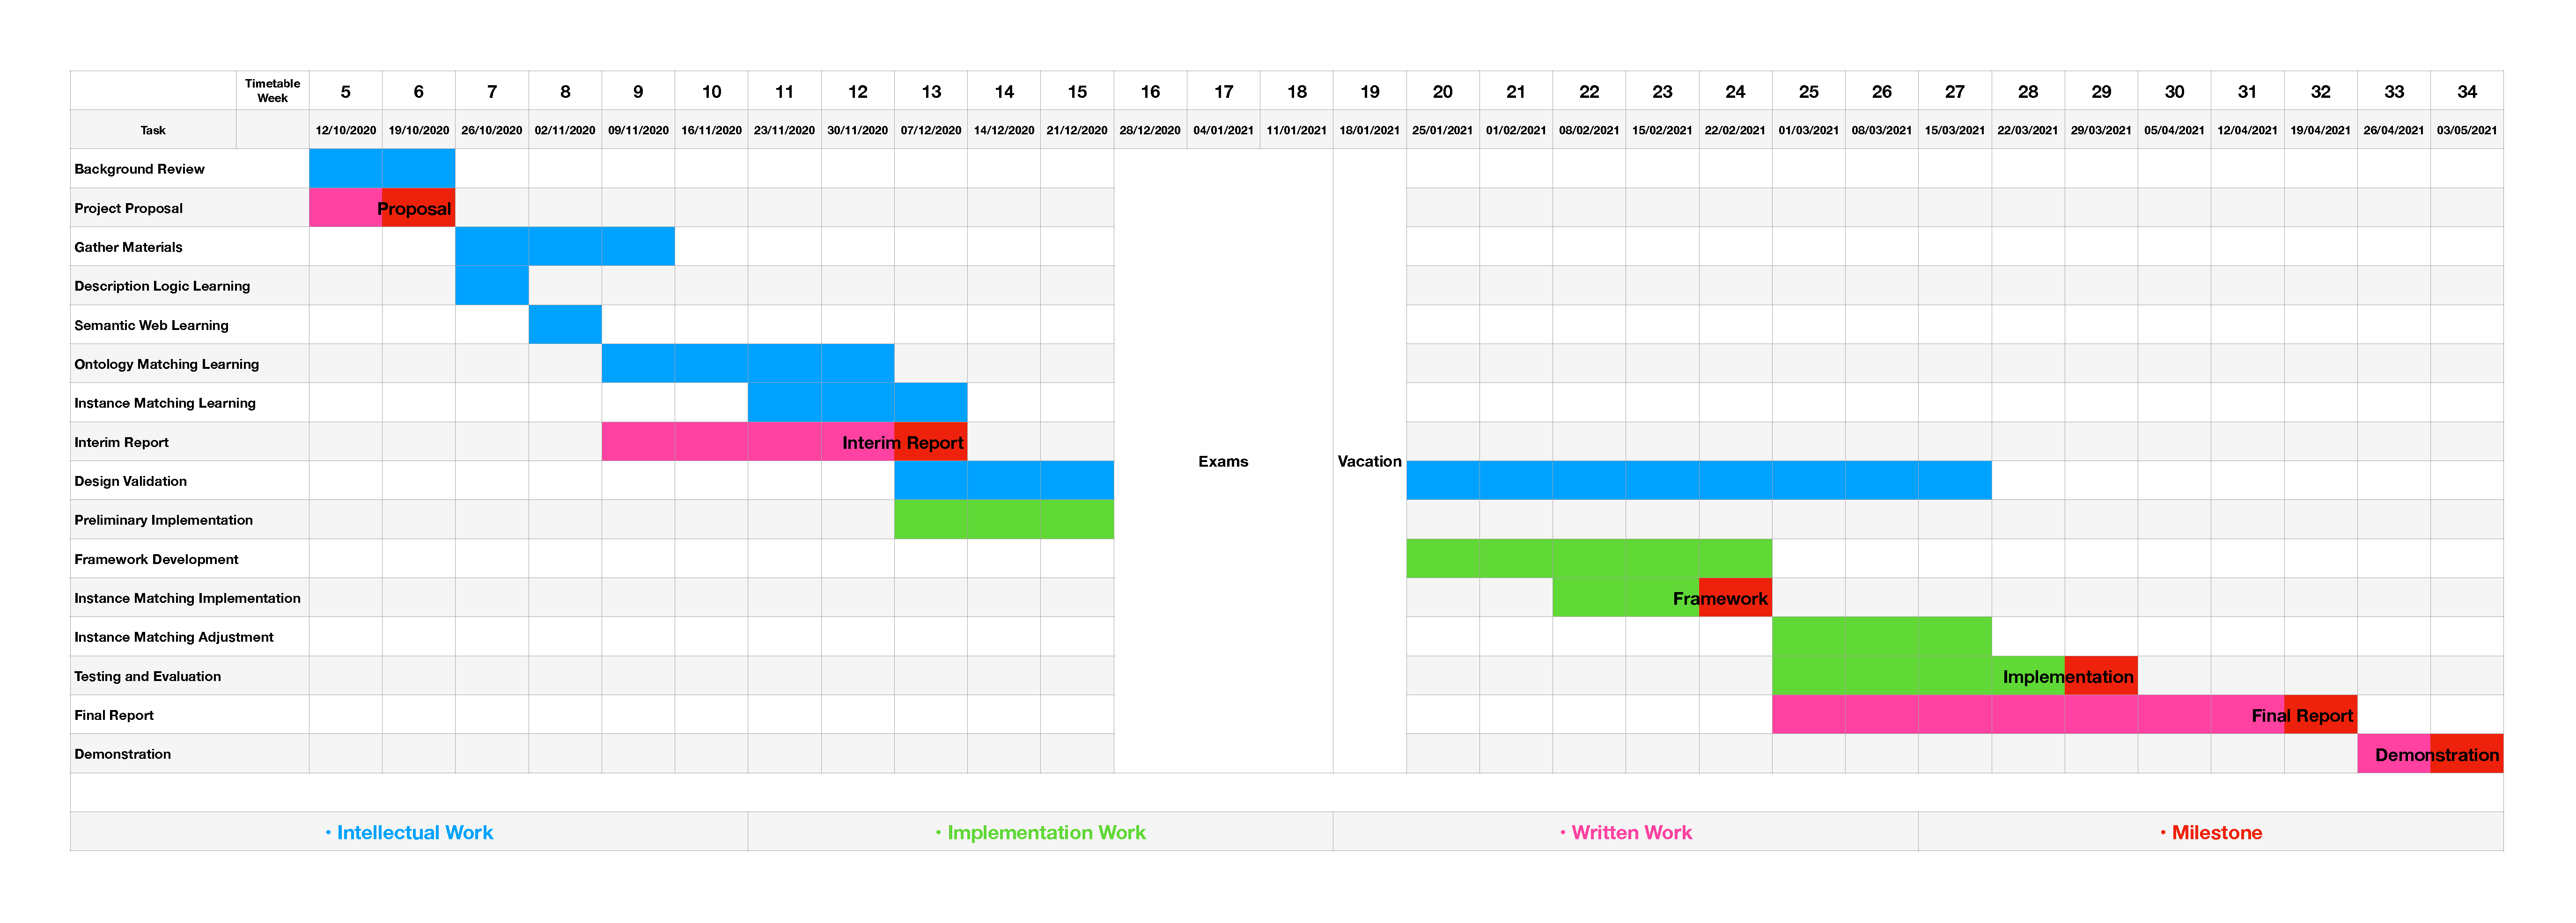
\includegraphics[width=\textwidth]{img/Gantt_new.pdf}
\caption{Revised workplan}
\label{fig:Gantt_new}
\end{subfigure}
\caption{Revision of workplan}
\label{fig:Gantt}
\end{figure}

\subsection{Working Methodology}
% Scrumban methodology.
While the workplan is designed with respect to the Waterfall methodology \cite{balaji2012waterfall} for clear validation of progress against the milestones, a hybrid combination of the Scrum and Kanban methodologies, namely Scrumban \cite{DBLP:conf/ispw/NikitinaKS12}, was adopted and followed as the working methodology since the beginning. The Scrum aspect splits the workload into small, easily achievable goals which could be reviewed regularly, while a Kanban board enables clear monitoring of the process, with tasks being assigned in dynamic \textquotedblleft lanes\textquotedblright \space (see figure \ref{fig:Kanban}). Fusing the two together exploits the advantages of both: the workflow can adapt to changes quickly, and since all tasks are visualised, the efforts can be well balanced and coordinated. The sprint interval for Scrumban was set to 1 week, which is the interval between every consecutive meetings with my supervisor. This helped tremendously in pushing everything forward, so that the project can progress at a good pace despite the intense curricular work during the fall semester and my lack of experience in carrying out a large project like this individually.

\begin{figure}[ht]
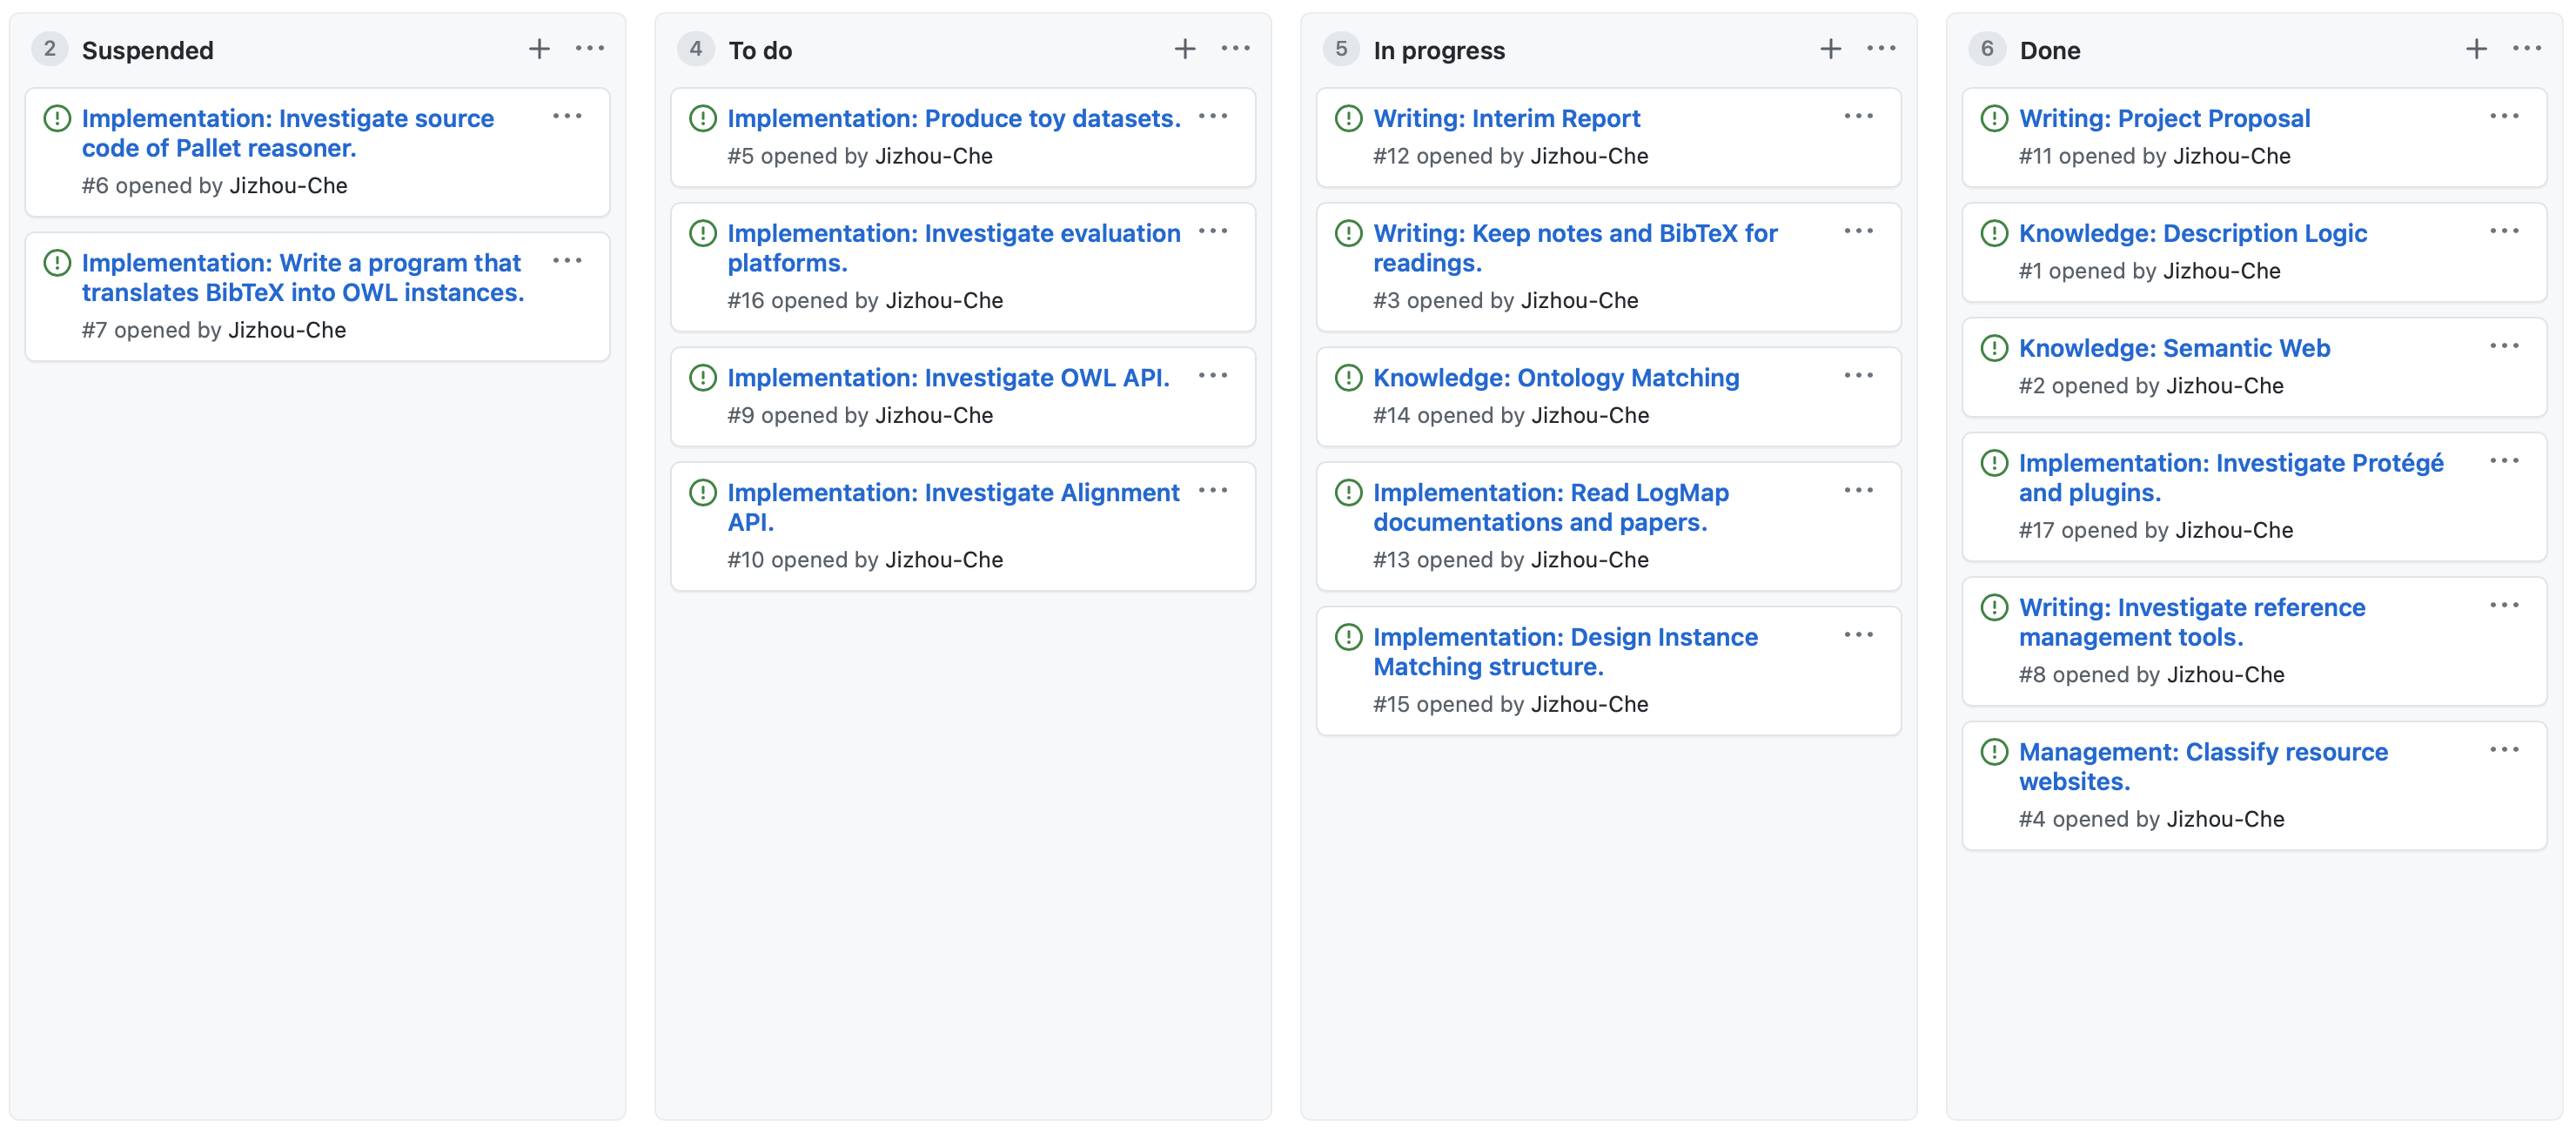
\includegraphics[width=\textwidth]{img/Kanban.png}
\caption{Kanban board}
\label{fig:Kanban}
\end{figure}

\subsection{Resource Management}
% Resource management.
All resources related to the project, such as meeting minutes, reading notes and source code have been managed with the Git version control system and consistently pushed to GitHub. They can be found at \url{https://github.com/Jizhou-Che/Dissertation}. This has proven to be a good practice, in that the evolution of the project is documented within the accumulation and development of resources. The project will stick closely to this methodology during its second half.

\subsection{Contingency Measures}
% Risks that may arise in the revised workplan, and how they can be mitigated and managed.
Admittedly, I did not put too much thought into contingency measures at the start of the project. However, I have learned its necessity though my experience in managing this long-term project. Based on the issues I have encountered in the first part of the project as well as my personal observations, the most significant risks that can arise in the process are pointed out below, as well as the proposed strategies to mitigate their effects.
\\\\
Underestimating the steepness of learning curves or the difficulty of implementation can disrupt the regular time allocation, and therefore shake the entire workplan. Apart from foreseeing the issue and allocate adequate amount of time in advance, time can be borrowed from flexible tasks that are less affected by a shrink of timespan. While this provides a temporary solution that mitigates the impact to the workplan, ultimately extra time should be dedicated to the project as compensation.
\\\\
The workloads of other modules is another serious issue, especially when their deadlines are close to the project milestones. This can not only disrupt the time management, but also increase the psychological pressure. Low moods and anxiety can lead to a drop in the productivity as well as the quality of work produced. Having tried the relax-then-focus approach, that was not suitable for me as the guilty only increased. Instead, trying to finish the work together with a friend has proved to be more effective.
\\\\
Offline meetings can sometimes be inappropriate due to wellbeing or other issues. In such cases online meetings via Zoom were organised, and have proven equal effectiveness.


\section{Reflections}
% A personal reflection on the plan and your experience of the project (a critical appraisal of how the project went).
I have faced challenges in various aspects of the project. Academically, the steep learning curve of background knowledge made the workload even heavier during the term time that was already intense, and the locating of quality resources required profession judgment and guidance especially at the beginning. My supervisor helped me a lot in such aspects, so I could quickly dive into solid work. Regarding the management of the project, time allocation was the largest difficulty I encountered, as it was hard to balance the project with other curricular subjects, and sometimes my judgment of the amount of time required for a task was inadequate. I consider this as a necessary stage that must be gone through to toughen my skills and enrich my experience, and I feel I have made advancements in my abilities after the first half of the project.
\\\\
During the meetings with my supervisor, I have been taking an orienting role, by preparing relevant materials and questions before the meetings. This made sure that every meeting could go smoothly, and the contents are fully relevant to my working stage at that time. It was an engaging way to gain insights into my performance, and to help me get back on track when I encountered academic or project management difficulties. Thanks to the high quality of the meetings, I can maintain a strong motivation and a high productivity throughout. The meetings were also found to be a good opportunity for both my supervisor and I to know each other better. These are invaluable points and should definitely be kept during the upcoming stages.


\addcontentsline{toc}{chapter}{Bibliography}
\bibliographystyle{IEEEtran}
\bibliography{report}

\begin{appendices}

% e.g., User Manuals, supporting evidence for claims made in the main part of the dissertation (e.g. a copy of a user evaluation questionnaire), samples of test data, etc. Note that Appendices are optional.

\chapter{User Manuals}

\chapter{User Evaluation Questionnaire}

\end{appendices}


\end{document}
